%%%%%%%%%%%%%%%%%%%%%%%%%%%%%%%%%%%%%%%%%%%%%%%%%%%%%%%%%%%%%%%%%%%%%%%%%%%%%%%%
% Template for USENIX papers.
%
% History:
%
% - TEMPLATE for Usenix papers, specifically to meet requirements of
%   USENIX '05. originally a template for producing IEEE-format
%   articles using LaTeX. written by Matthew Ward, CS Department,
%   Worcester Polytechnic Institute. adapted by David Beazley for his
%   excellent SWIG paper in Proceedings, Tcl 96. turned into a
%   smartass generic template by De Clarke, with thanks to both the
%   above pioneers. Use at your own risk. Complaints to /dev/null.
%   Make it two column with no page numbering, default is 10 point.
%
% - Munged by Fred Douglis <douglis@research.att.com> 10/97 to
%   separate the .sty file from the LaTeX source template, so that
%   people can more easily include the .sty file into an existing
%   document. Also changed to more closely follow the style guidelines
%   as represented by the Word sample file.
%
% - Note that since 2010, USENIX does not require endnotes. If you
%   want foot of page notes, don't include the endnotes package in the
%   usepackage command, below.
% - This version uses the latex2e styles, not the very ancient 2.09
%   stuff.
%
% - Updated July 2018: Text block size changed from 6.5" to 7"
%
% - Updated Dec 2018 for ATC'19:
%
%   * Revised text to pass HotCRP's auto-formatting check, with
%     hotcrp.settings.submission_form.body_font_size=10pt, and
%     hotcrp.settings.submission_form.line_height=12pt
%
%   * Switched from \endnote-s to \footnote-s to match Usenix's policy.
%
%   * \section* => \begin{abstract} ... \end{abstract}
%
%   * Make template self-contained in terms of bibtex entires, to allow
%     this file to be compiled. (And changing refs style to 'plain'.)
%
%   * Make template self-contained in terms of figures, to
%     allow this file to be compiled. 
%
%   * Added packages for hyperref, embedding fonts, and improving
%     appearance.
%   
%   * Removed outdated text.
%
%%%%%%%%%%%%%%%%%%%%%%%%%%%%%%%%%%%%%%%%%%%%%%%%%%%%%%%%%%%%%%%%%%%%%%%%%%%%%%%%

\documentclass[letterpaper,twocolumn,10pt]{article}
\usepackage{usenix-2020-09}

% to be able to draw some self-contained figs
\usepackage{tikz}
\usepackage{amsmath}
\usepackage{algorithm}
\usepackage{algorithmic}

% inlined bib file
\usepackage{filecontents}

%-------------------------------------------------------------------------------
%-------------------------------------------------------------------------------
\begin{document}
%-------------------------------------------------------------------------------


% make title bold and 14 pt font (Latex default is non-bold, 16 pt)
\title{VGuardDB: An Extension of VGuard for Efficiently Storing and Accessing Data from V2X Networks}

\maketitle

\begin{abstract}
VGuard proposes a new permissioned blockchain that achieves consensus for vehicular data under changing memberships. However, VGuard only produces chained consensus results of data entries but does not store them in a database but only on a log file, making it challenging to retrieve data from the blockchain for analysis and decision-making. Additionally, the VGuard paper has not specified the structure of the supported data entries or the use cases that generate them. To address these issuses, we introdudce VGuardDB, which adds a database layer to VGuard, where each vehicle has a distributed database to store data, provide access to the agreed data through the read capabilities of the database layer and define specific data structures. As such, the proposed enhancements to the VGuard blockchain system will enable an efficient and reliable data storage and retrieval, improving the usability of the system and enhancing its practical application.
\end{abstract}
\begin{figure*}[t]
    \centering
    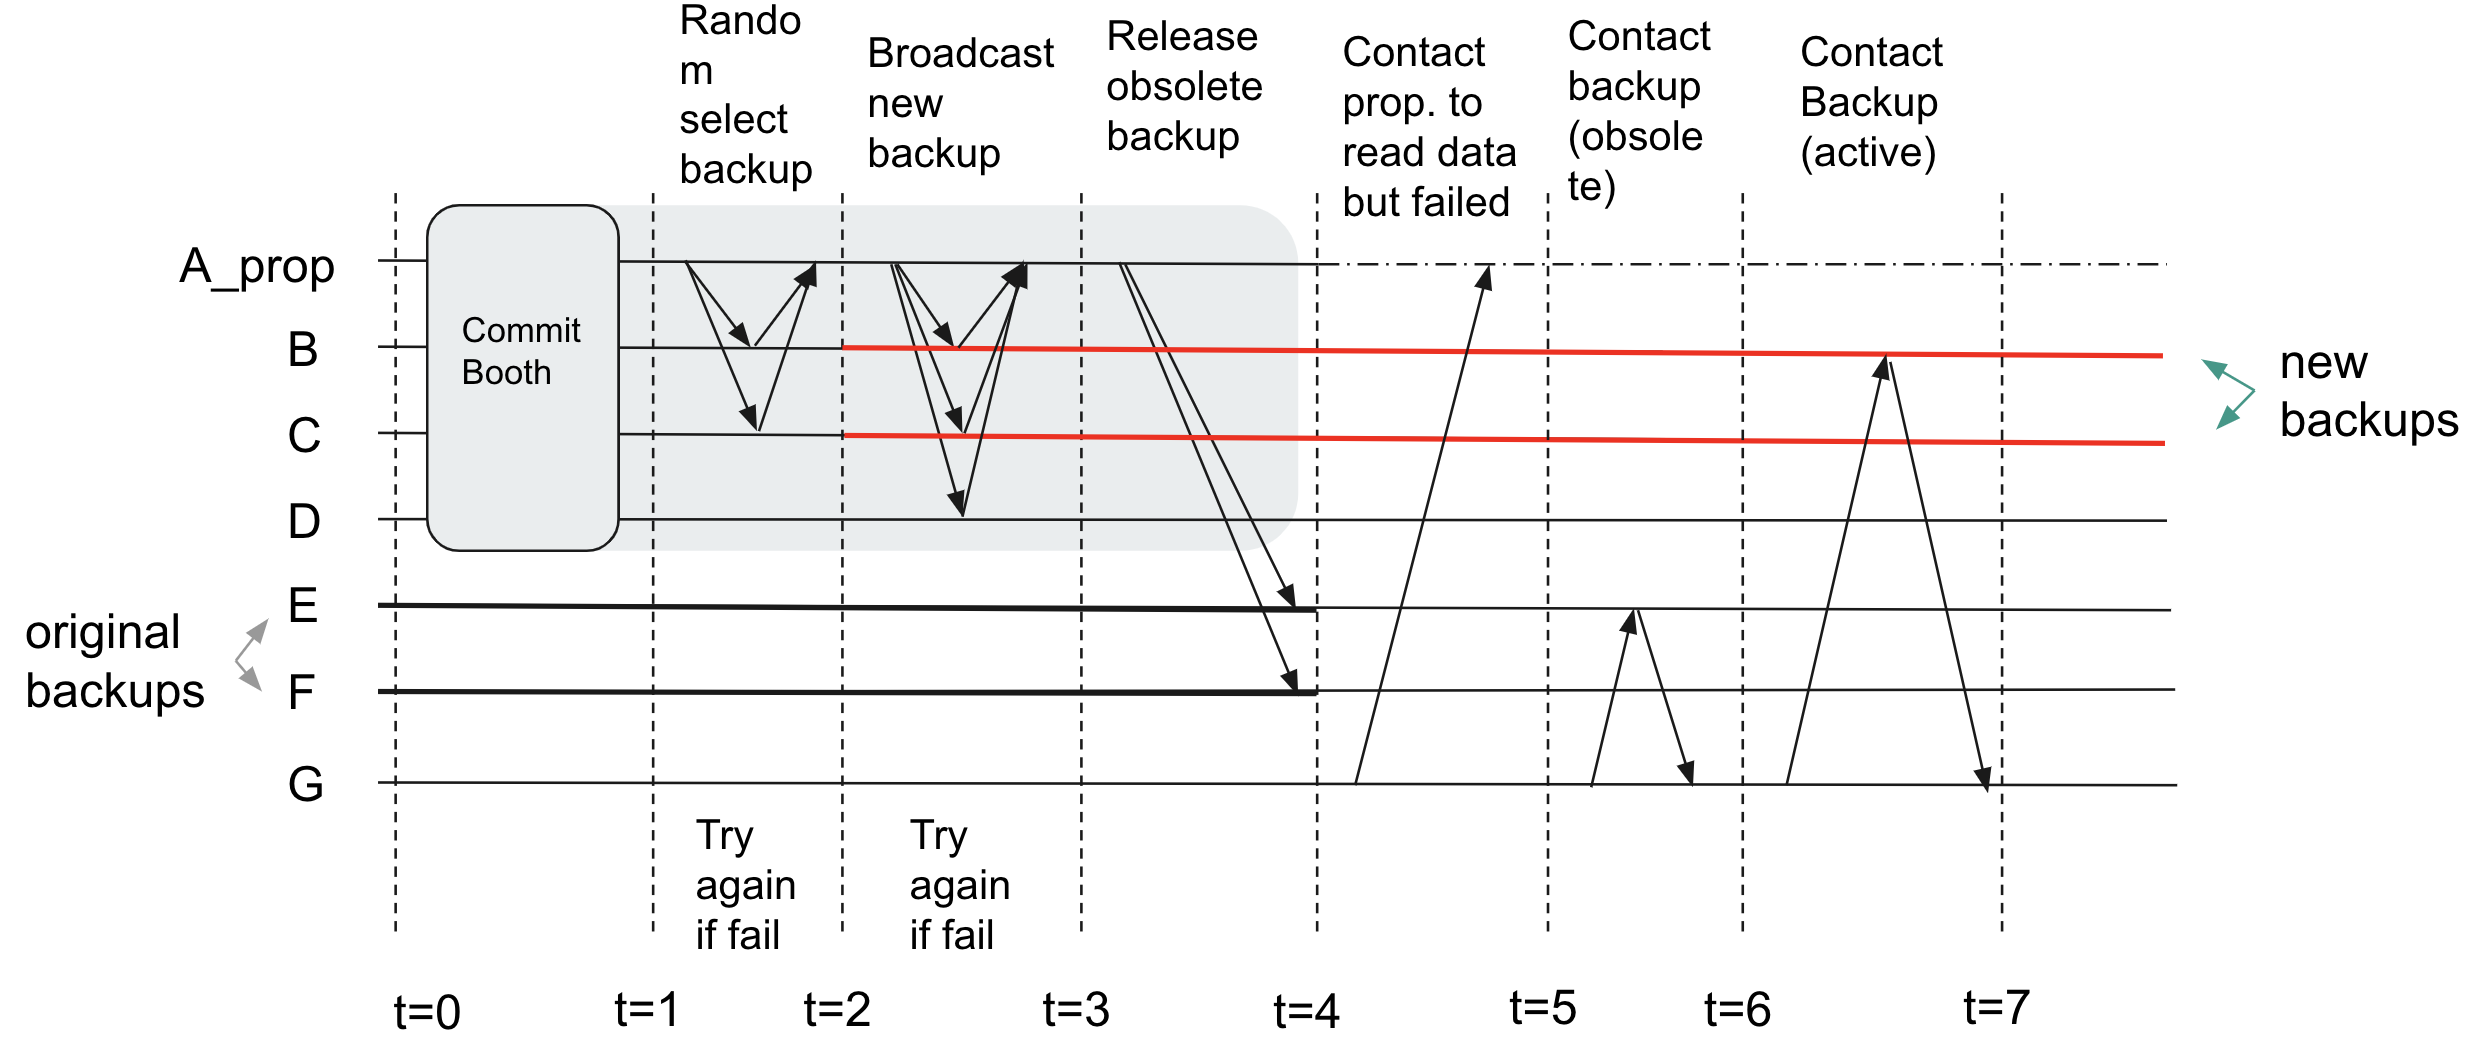
\includegraphics[width=\textwidth]{img/worflow.png}
    \caption{The overall workflow of VGuardDB, illustrated with an example of one proposer (A) and six validators (B to G). At t=0, A hosts a commit booth with B, C, and D. E, and F are vehicles that are chosen as backups from a previous booth. The back-up replication phase is triggered at t=1, when the commit booth ends. A first randomly chooses B and C to be backups, and upon success, broadcast the information to vehicles in the booth. A then startes the data-release phase by informing E and F that they are no longer the backups, and are now free to delete their local data. At t=4, Vehicle G initializes the read phase by sending a read request to A. By default, all vehicles are configured to read from the proposer first, but in this case, A has gone offline (as illustrated in dashed line), so G attemps to read from of the backups according to its local backup list. Since G is not informed that B and C are the current active backups, it makes the request to E, one of the now obsolete backups. E then informs G that B is the active backup, and G makes the request to B. B then informs G that it has the data, and G receives the data. }
    \label{fig:workflow}
\end{figure*}
\section{Introduction}
With the quickly growing popularity of smart vehicles as well as smart transportation systems, the need for efficient and reliable communication between vehicles and the surrounding infrastructure is becoming more and more important. Vehicle-to-everything (V2X) communication is a promising technology that enables vehicles to communicate with each other and the surrounding infrastructure, such as traffic lights, road signs, and other vehicles. V2X communication can be used to improve road safety, reduce traffic congestion, and improve the efficiency of transportation systems. 

However, the vast amount of data generated by V2X networks are often unaccessible to users and monopolized by auto manufacturers. In response, there has been an increasing demand for a distributed data storage option for V2X data. However, the unpredictable dynamic nature of road and vehicle conditions renders applying traditional distributed data storage solutions such as blockchians difficult in a V2X environment. To address these issues, VGuard[] has been proposed as a permissioned blockchain that achieves consensus for vehicular data under changing memberships. VGuard is designed to be used in V2X networks, where the consensus is achieved by the vehicles in the network. However, VGuard only produces chained consensus results of data entries but does not store them in a database but only on a log file, making it challenging to retrieve data from the blockchain for analysis and decision-making. Additionally, the VGuard paper has not specified the structure of the supported data entries or the use cases that generate them. 

To fill in this missing component, we introduce VGuardDB, which creates and additional database layer on top of VGuard, where each vehicle has a distributed database to store data, provide access to the agreed data through the read capabilities of the database layer and define specific data structures. VGuardDB ensures data avaialbility as long as a the number the number of unavaible vehicles, including the proposer, is smaller than a configurable value. Additionally, we disign VGuardDB such that only the configured number of randomly selected vehicles need to store data on the chain at any given point in time, in order to save storage space on vehicles. As such, the proposed enhancements to the VGuard blockchain system will enable an efficient and reliable data storage and retrieval, improving the usability of the system and enhancing its practical application.

The rest of the paper is organized as follows. Section 2 provides an overview of related work in the field. Section 3 describes the architecture and design of VGuardDB, including the extension of VGuard, the storage layer, and the use of MySQL. Section 4 presents the experimental results and evaluation of VGuardDB's performance. Finally, Section 5 concludes the paper and outlines future research directions.

\section{Related Work}
There have been some existing works that aim to create a fusion between blockchain and distributed databases in order to combine the advantages of both worlds. BlockchainDB[1] proposes a novel architecture that uses a scalable and efficient database as a storage layer and a blockchain as an append-only log that records the history of data modifications. Another example is Blockchain Relational Database (BRD)[2], a novel architecture for a blockchain relational database that leverages the rich features of a replicated relational database and extends them with blockchain properties such as immutability, provenance, and consensus.
Regarding the applicability of V2X blockchain technology, some research works have analyzed and categorized some real use-case scenarios. For example,  [3] presents a taxonomy of design use cases and system architectures for blockchain applications in V2X communication and discusses how blockchains can be used to record and distribute data such as software updates, driver behaviors, and accident reports among different stakeholders. 

\section{Design}
The core logic of VGuardDB can be divided to 3 independent phases, which are the backup-replication phase, the data-release phase, and the data-read phase. The backup-replication phase is responsible for making backups of the data on the chain. The data-release phase is responsible for releasing data from obsolete replicates. The data-read phase is responsible for reading the data from the database. The overall workflow is illustrated in figure \ref{fig:workflow}. The following subsections describe the design of each phase in detail.

\subsection{Backup-Replication Phase}
The backup-replication phase is responsible for making backup database on the chain. The backup-replication phase is triggered when at the end of the commit consensus phase in VGuard. Upon which, VGuard sends a request to VGuardDB to make backups of the data on the chain. VGuardDB then randomly selects a number of vehicles from the current participants in the commit consensus phase, and sends a request to each of them to make a backup of the data on the chain. If the request is successful, VGuardDB then sends a request to the proposer to broadcast the information of the new backups to the vehicles that participated the commit consensus booth. The vehicles then update their local backup list with the new backups.

The following pseudocode illustrates the logic of the \texttt{backup\_replication} function:

\begin{algorithm}[H]
\caption{backup\_replication(payload, conn)}
\begin{algorithmic}
\STATE $status \gets \text{False}$
\STATE $participants \gets payload['participants']$
\STATE $backup\_list \gets current\_backup\_list $
\WHILE{$\text{not } status$}
    \STATE $status, chosen \gets \text{make\_random\_backups}(participants, conn)$
    \IF{$\text{not } status$}
        \STATE \textbf{continue}
    \ENDIF
    \STATE $status \gets \text{broadcast\_backups\_to\_booth}(chosen, participants)$
    \STATE $backup\_list \gets \text{update\_backup\_list}(chosen, backup\_list)$
    \STATE $\text{request\_delete\_obsolete(backup\_list)}$
\ENDWHILE
\end{algorithmic}
\end{algorithm}

\subsection{Data-Release Phase}

\subsection{Data-Read Phase}
\section{Implementation}
We design VGuardDB in a way that it can be easily integrated into existing VGuard implementations in a modular fashion. The architecture of VGuardDB is shown in Figure \ref{fig:architecture}. The VGuardDB architecture consists of three main components: A Python Flask-based API, A main logic layer, and a MySQL-based data storage layer. The API layer is responsible for receiving requests from the vehicles and forwarding them to the main logic layer. The main logic layer is responsible for the main logic of the system, including making database replicas as well as handling data-read functionality. The storage layer is responsible for storing the data and is shared with VGuard.


\section{Evaluation}
%%%%%%%%%%%%%%%%%%%%%%%%%%%%%%%%%%%%%%%%%%%%%%%%%%%%%%%%%%%%%%%%%%%%%%%%%%%%%%%%
\end{document}
%%%%%%%%%%%%%%%%%%%%%%%%%%%%%%%%%%%%%%%%%%%%%%%%%%%%%%%%%%%%%%%%%%%%%%%%%%%%%%%%

%%  LocalWords:  endnotes includegraphics fread ptr nobj noindent
%%  LocalWords:  pdflatex acks